\chapter{Additional \gls{PNN} Score Plots}\label{app:pnn-scores}

	\clearpage
	\section{\taujets PNN Scores}\label{sec:taujet-pnn-scores}
		\clearpage
		\begin{figure}
		  \centering
			\subfloat[\label{fig:taujets_SR_PNNscores_app_1_a}]{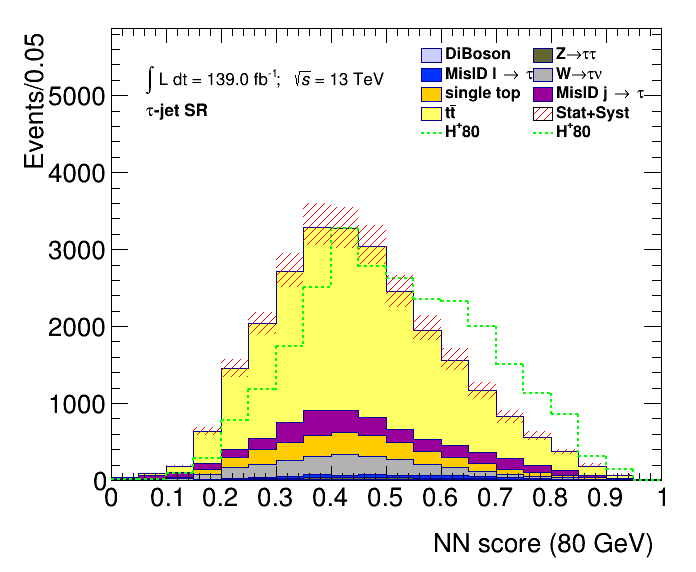
\includegraphics[width=0.45\linewidth]{chapters/chapter6_HPlus/images/taujets/clf_score_GB200_mass_80to80_SR_TAUJET.png}}
			\subfloat[\label{fig:taujets_SR_PNNscores_app_1_b}]{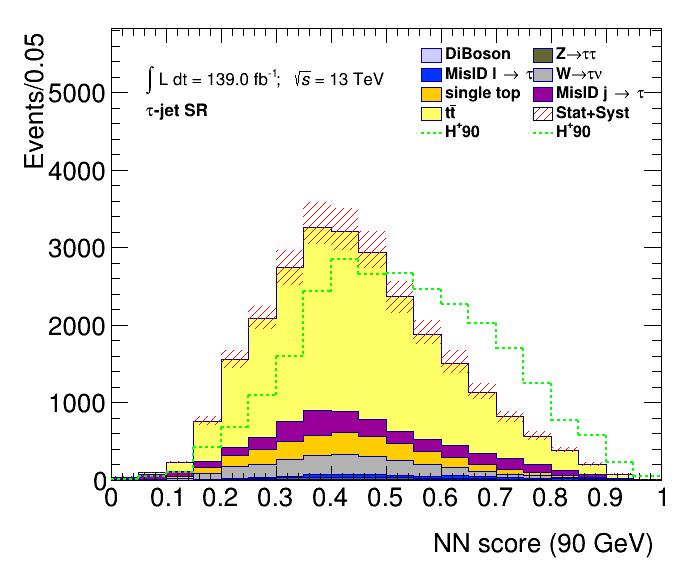
\includegraphics[width=0.45\linewidth]{chapters/chapter6_HPlus/images/taujets/clf_score_GB200_mass_90to90_SR_TAUJET.png}} \\
			\subfloat[\label{fig:taujets_SR_PNNscores_app_1_c}]{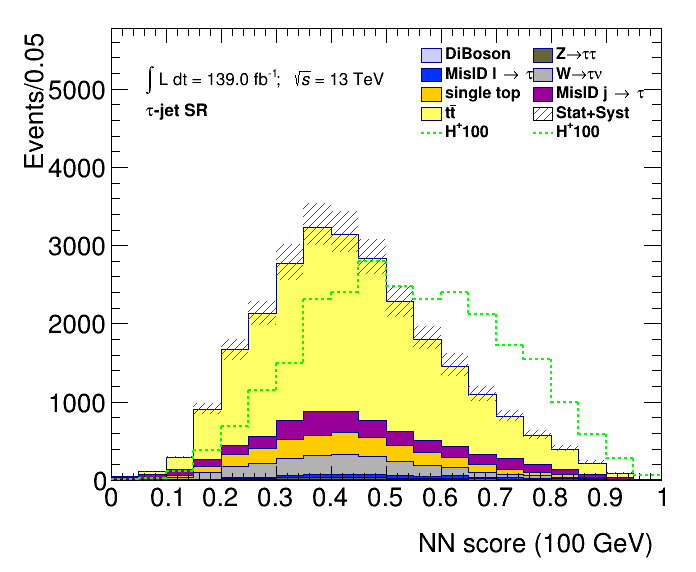
\includegraphics[width=0.45\linewidth]{chapters/chapter6_HPlus/images/taujets/clf_score_GB200_mass_100to100_SR_TAUJET.png}}
			\subfloat[\label{fig:taujets_SR_PNNscores_app_1_d}]{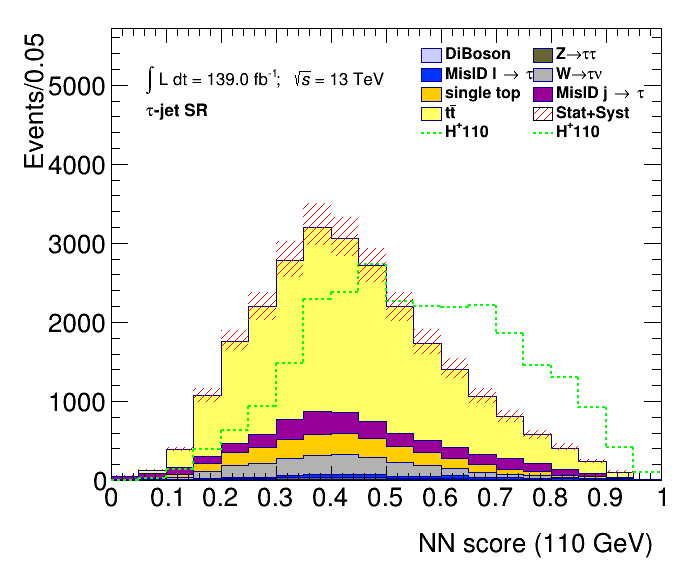
\includegraphics[width=0.45\linewidth]{chapters/chapter6_HPlus/images/taujets/clf_score_GB200_mass_110to110_SR_TAUJET.png}} \\
			\subfloat[\label{fig:taujets_SR_PNNscores_app_1_e}]{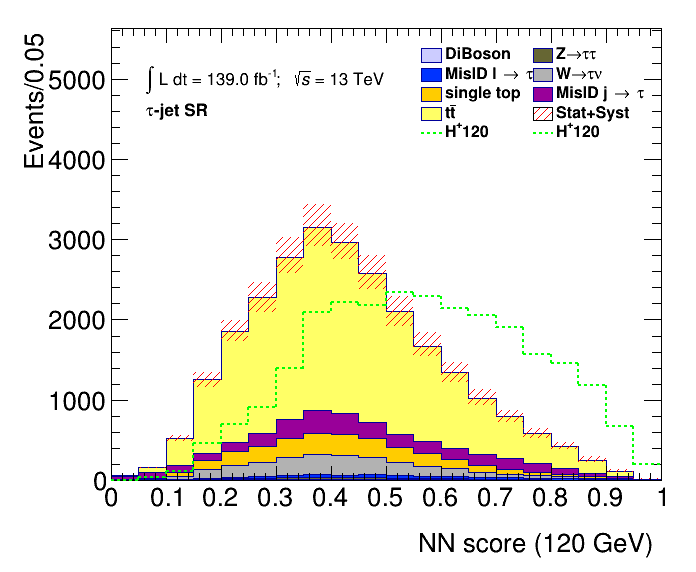
\includegraphics[width=0.45\linewidth]{chapters/chapter6_HPlus/images/taujets/clf_score_GB200_mass_120to120_SR_TAUJET.png}}
			\subfloat[\label{fig:taujets_SR_PNNscores_app_1_f}]{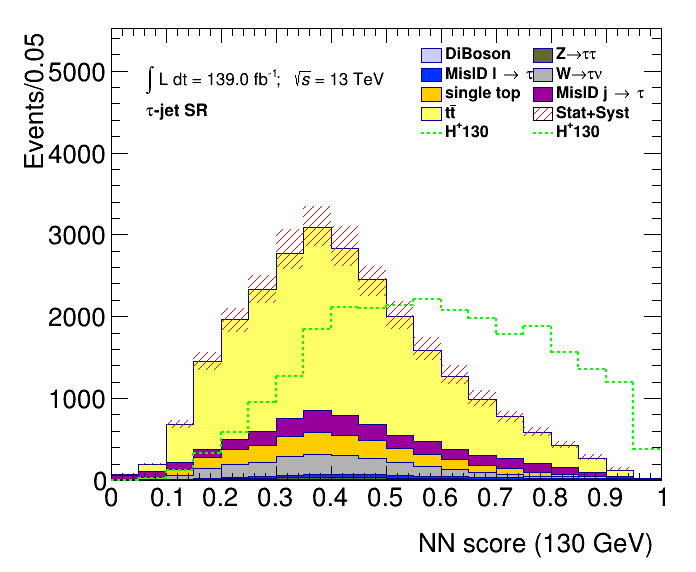
\includegraphics[width=0.45\linewidth]{chapters/chapter6_HPlus/images/taujets/clf_score_GB200_mass_130to130_SR_TAUJET.png}}
			  \caption{\label{fig:taujets_SR_PNNscores_app_1} \gls{PNN} score distributions in the
			signal region of the \taujets channel, for the six charged Higgs boson mass parameters.
			 The uncertainty bands include all statistical and systematic uncertainties. 
			The normalization of the signal (shown for illustration) corresponds to the integral of the background.}
		\end{figure}

		\begin{figure}
		  \centering
			\subfloat[\label{fig:taujets_SR_PNNscores_app_2_a}]{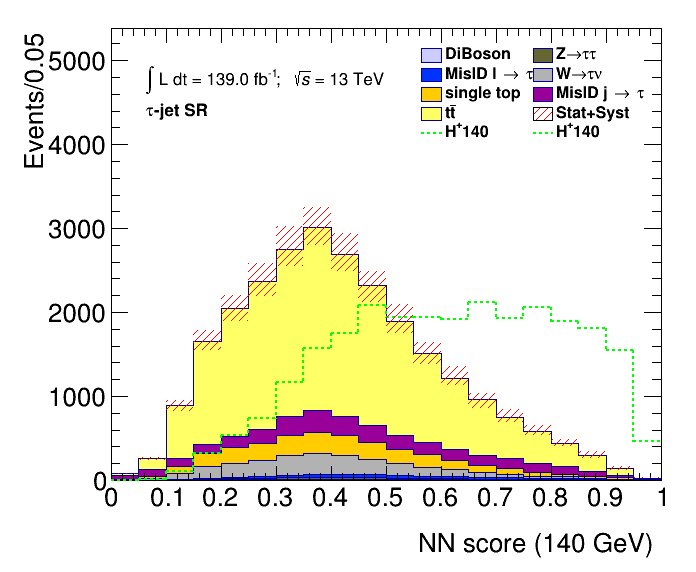
\includegraphics[width=0.45\linewidth]{chapters/chapter6_HPlus/images/taujets/clf_score_GB200_mass_140to140_SR_TAUJET.png}}
			\subfloat[\label{fig:taujets_SR_PNNscores_app_2_b}]{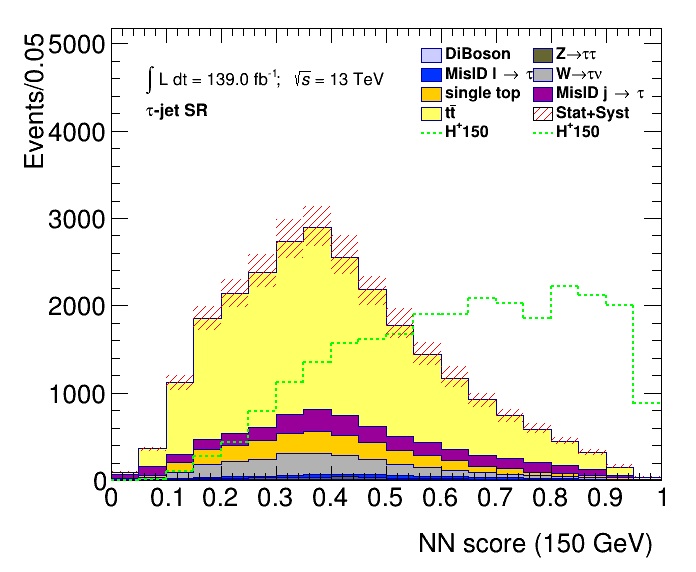
\includegraphics[width=0.45\linewidth]{chapters/chapter6_HPlus/images/taujets/clf_score_GB200_mass_150to150_SR_TAUJET.png}} \\
			\subfloat[\label{fig:taujets_SR_PNNscores_app_2_c}]{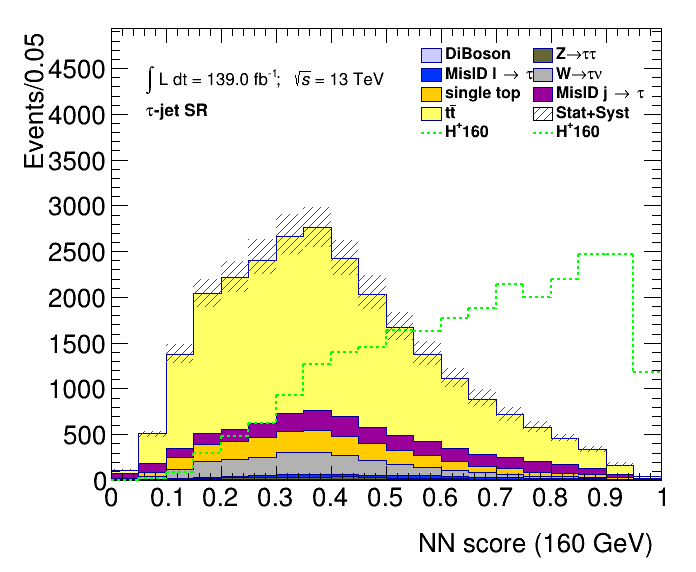
\includegraphics[width=0.45\linewidth]{chapters/chapter6_HPlus/images/taujets/clf_score_GB200_mass_160to160_SR_TAUJET.png}}
			\subfloat[\label{fig:taujets_SR_PNNscores_app_2_d}]{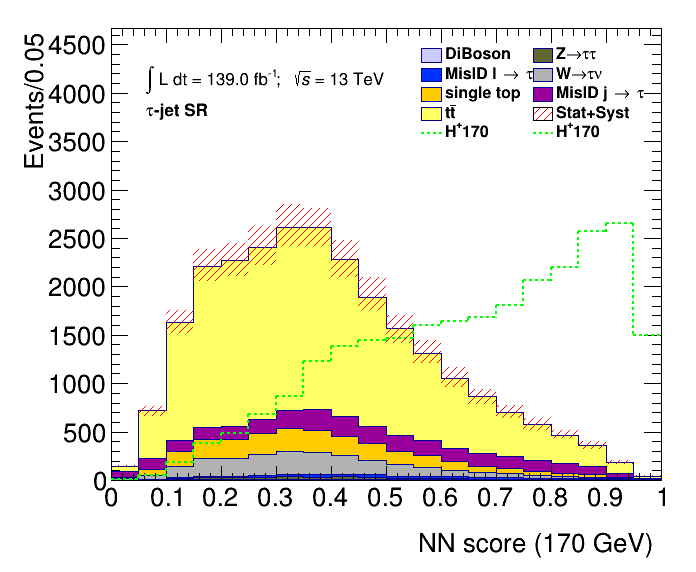
\includegraphics[width=0.45\linewidth]{chapters/chapter6_HPlus/images/taujets/clf_score_GB200_mass_170to170_SR_TAUJET.png}} \\
			\subfloat[\label{fig:taujets_SR_PNNscores_app_2_e}]{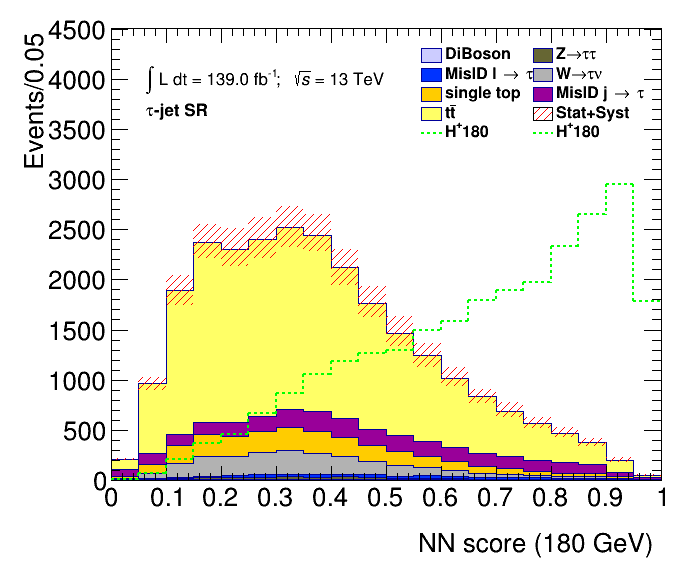
\includegraphics[width=0.45\linewidth]{chapters/chapter6_HPlus/images/taujets/clf_score_GB200_mass_180to180_SR_TAUJET.png}}
			\subfloat[\label{fig:taujets_SR_PNNscores_app_2_f}]{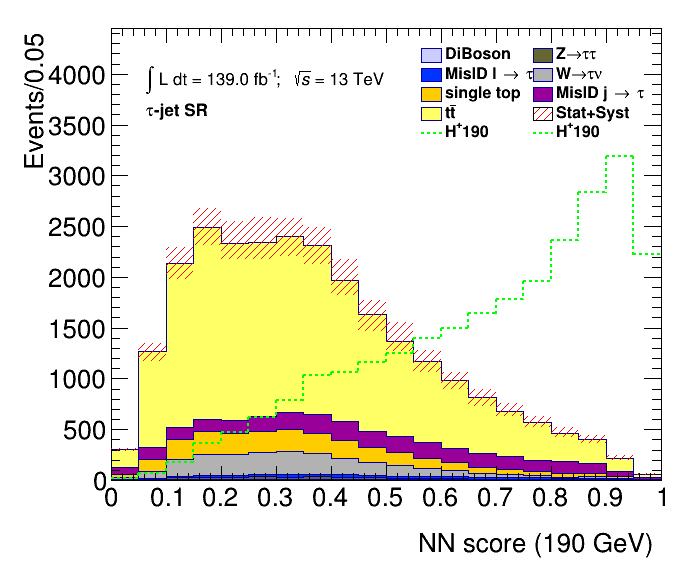
\includegraphics[width=0.45\linewidth]{chapters/chapter6_HPlus/images/taujets/clf_score_GB200_mass_190to190_SR_TAUJET.png}}
			  \caption{\label{fig:taujets_SR_PNNscores_app_2} \gls{PNN} score distributions in the
			signal region of the \taujets channel, for the six charged Higgs boson mass parameters.
			 The uncertainty bands include all statistical and systematic uncertainties. 
			The normalization of the signal (shown for illustration) corresponds to the integral of the background.}
		\end{figure}

		\begin{figure}
		  \centering
			\subfloat[\label{fig:taujets_SR_PNNscores_app_3_a}]{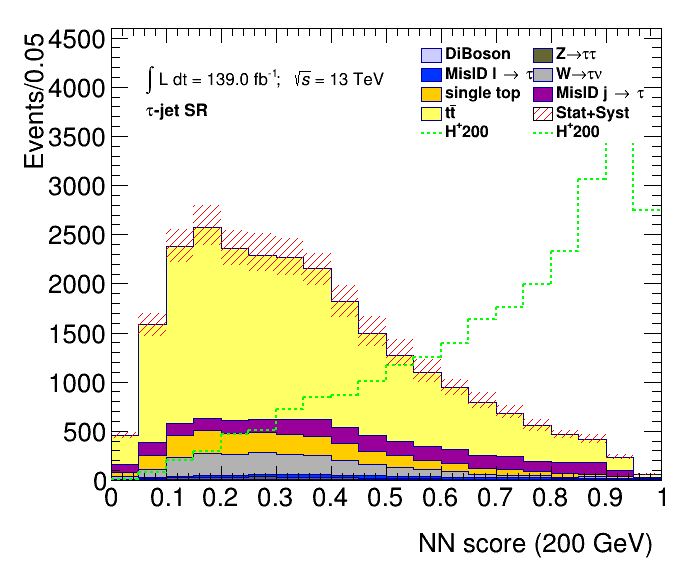
\includegraphics[width=0.45\linewidth]{chapters/chapter6_HPlus/images/taujets/clf_score_GB200_mass_200to200_SR_TAUJET.png}}
			\subfloat[\label{fig:taujets_SR_PNNscores_app_3_b}]{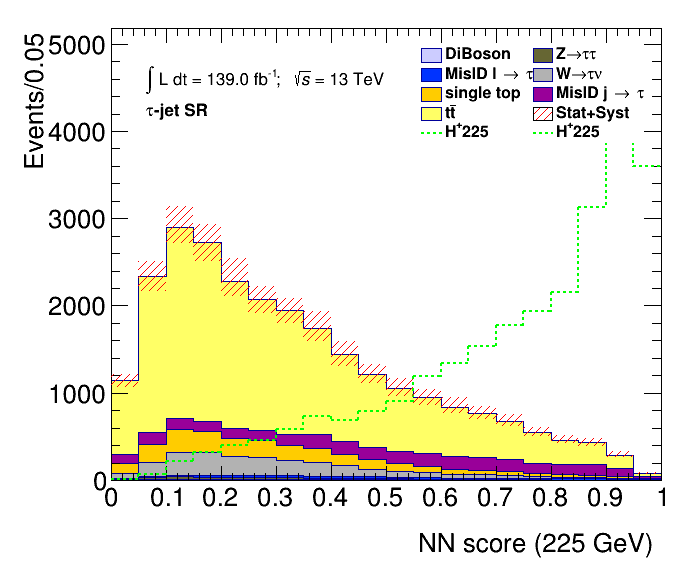
\includegraphics[width=0.45\linewidth]{chapters/chapter6_HPlus/images/taujets/clf_score_GB200_mass_225to225_SR_TAUJET.png}} \\
			\subfloat[\label{fig:taujets_SR_PNNscores_app_3_c}]{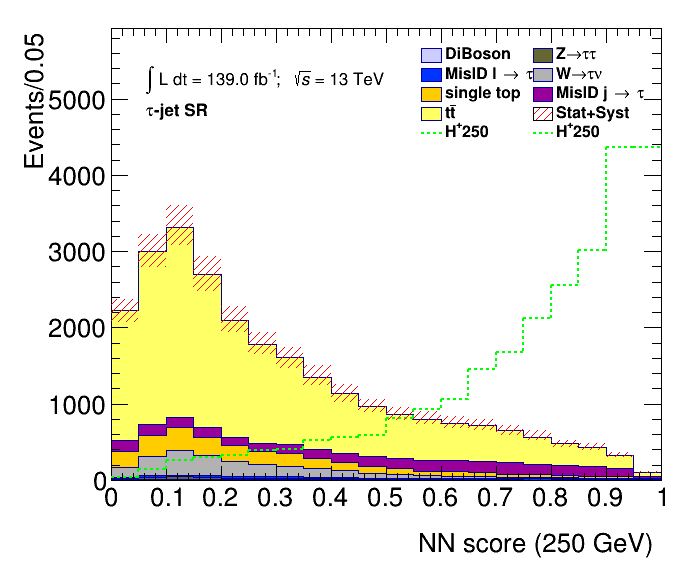
\includegraphics[width=0.45\linewidth]{chapters/chapter6_HPlus/images/taujets/clf_score_GB200_mass_250to250_SR_TAUJET.png}}
			\subfloat[\label{fig:taujets_SR_PNNscores_app_3_d}]{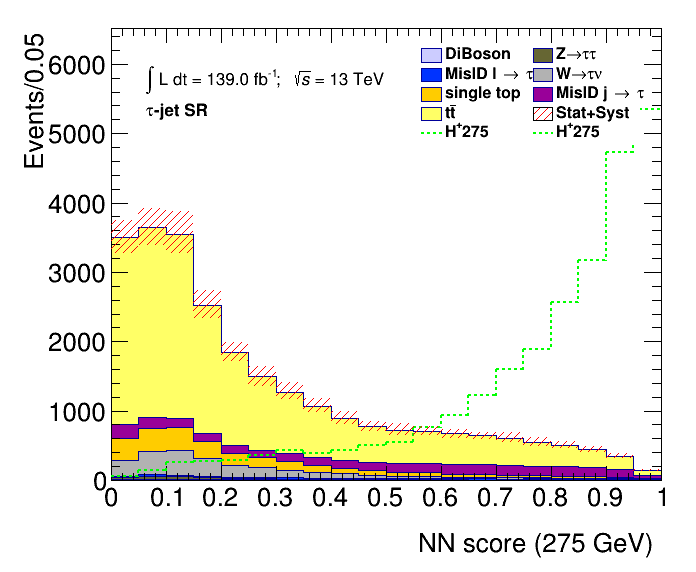
\includegraphics[width=0.45\linewidth]{chapters/chapter6_HPlus/images/taujets/clf_score_GB200_mass_275to275_SR_TAUJET.png}} \\
			\subfloat[\label{fig:taujets_SR_PNNscores_app_3_e}]{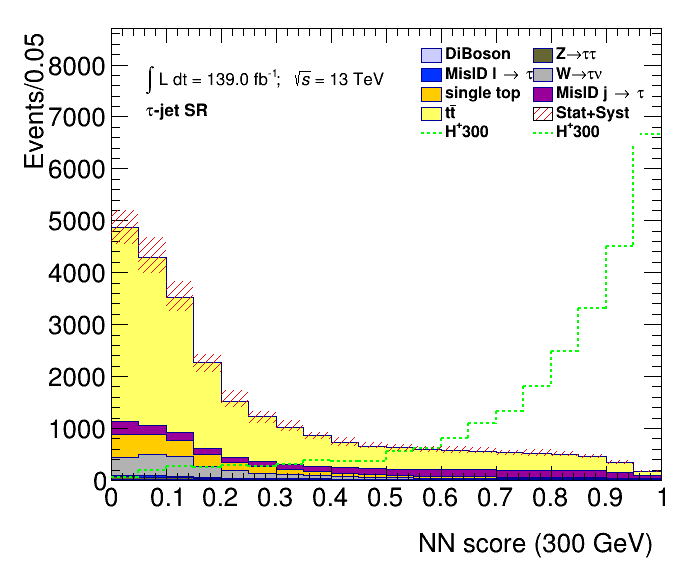
\includegraphics[width=0.45\linewidth]{chapters/chapter6_HPlus/images/taujets/clf_score_GB200_mass_300to300_SR_TAUJET.png}}
			\subfloat[\label{fig:taujets_SR_PNNscores_app_3_f}]{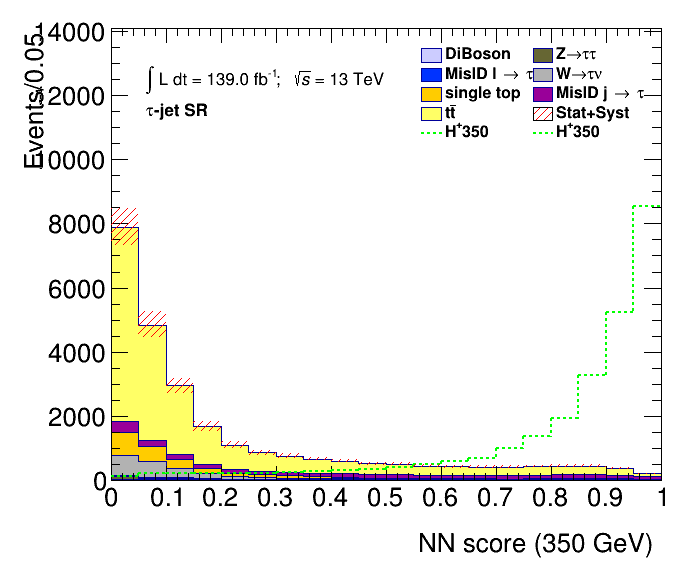
\includegraphics[width=0.45\linewidth]{chapters/chapter6_HPlus/images/taujets/clf_score_GB200_mass_350to350_SR_TAUJET.png}}
			  \caption{\label{fig:taujets_SR_PNNscores_app_3} \gls{PNN} score distributions in the
			signal region of the \taujets channel, for the six charged Higgs boson mass parameters.
			 The uncertainty bands include all statistical and systematic uncertainties. 
			The normalization of the signal (shown for illustration) corresponds to the integral of the background.}
		\end{figure}

		\begin{figure}
		  \centering
			\subfloat[\label{fig:taujets_SR_PNNscores_app_4_a}]{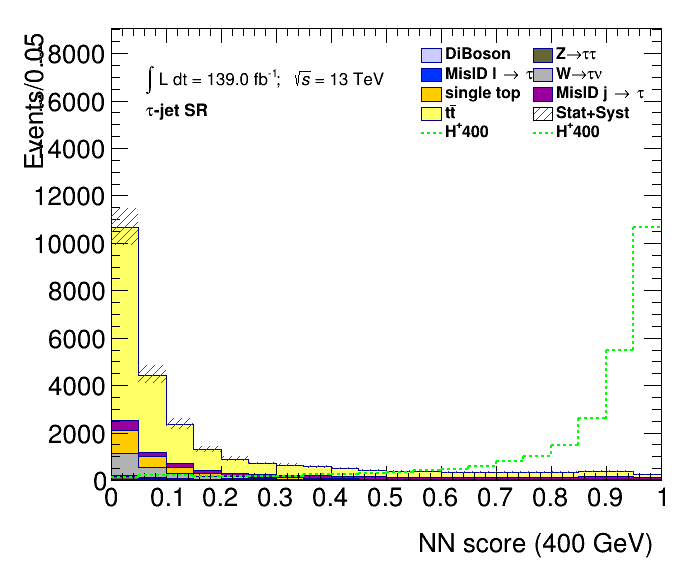
\includegraphics[width=0.45\linewidth]{chapters/chapter6_HPlus/images/taujets/clf_score_GB200_mass_400to400_SR_TAUJET.png}}
			\subfloat[\label{fig:taujets_SR_PNNscores_app_4_b}]{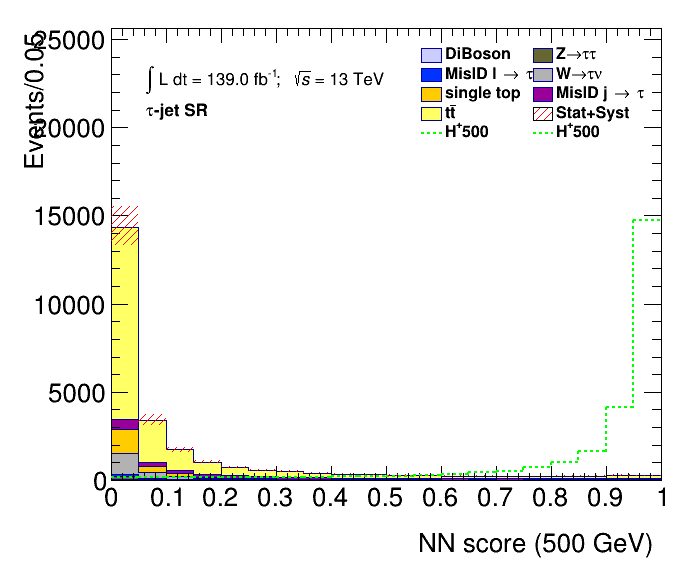
\includegraphics[width=0.45\linewidth]{chapters/chapter6_HPlus/images/taujets/clf_score_GB200_mass_500to500_SR_TAUJET.png}} \\
			\subfloat[\label{fig:taujets_SR_PNNscores_app_4_c}]{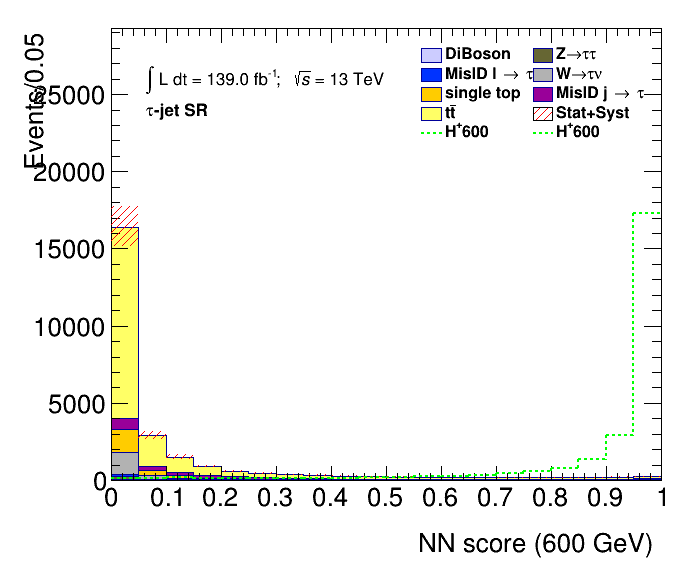
\includegraphics[width=0.45\linewidth]{chapters/chapter6_HPlus/images/taujets/clf_score_GB200_mass_600to600_SR_TAUJET.png}}
			\subfloat[\label{fig:taujets_SR_PNNscores_app_4_d}]{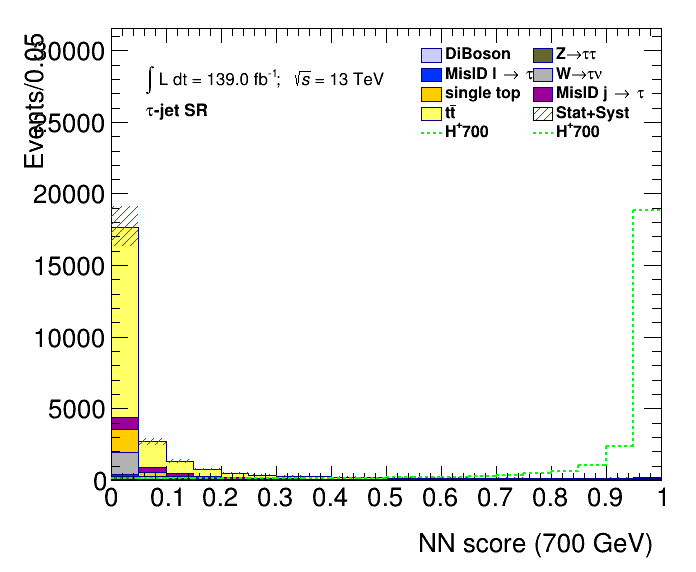
\includegraphics[width=0.45\linewidth]{chapters/chapter6_HPlus/images/taujets/clf_score_GB200_mass_700to700_SR_TAUJET.png}} \\
			\subfloat[\label{fig:taujets_SR_PNNscores_app_4_e}]{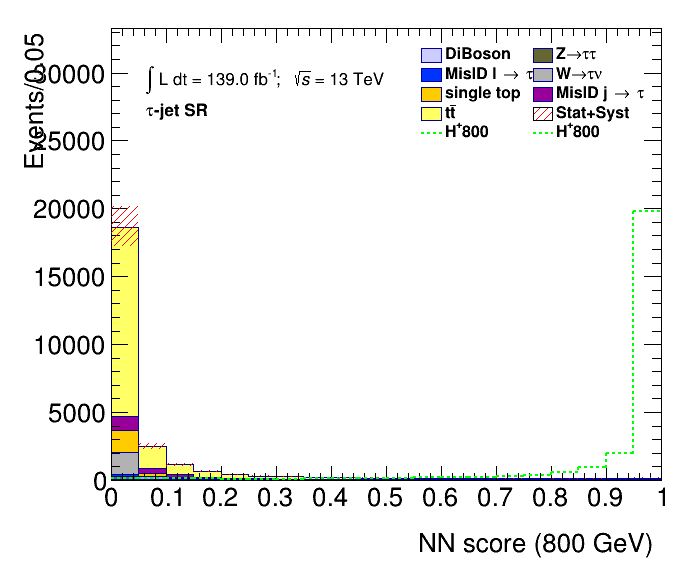
\includegraphics[width=0.45\linewidth]{chapters/chapter6_HPlus/images/taujets/clf_score_GB200_mass_800to800_SR_TAUJET.png}}
			\subfloat[\label{fig:taujets_SR_PNNscores_app_4_f}]{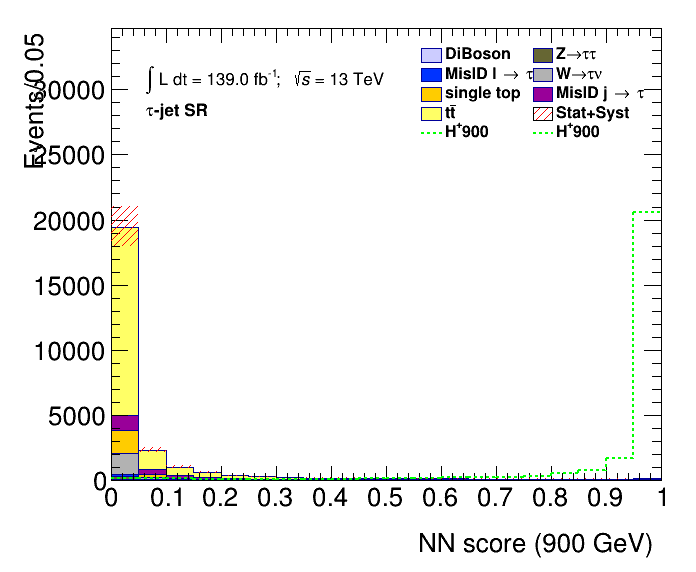
\includegraphics[width=0.45\linewidth]{chapters/chapter6_HPlus/images/taujets/clf_score_GB200_mass_900to900_SR_TAUJET.png}}
			  \caption{\label{fig:taujets_SR_PNNscores_app_4} \gls{PNN} score distributions in the
			signal region of the \taujets channel, for the six charged Higgs boson mass parameters.
			 The uncertainty bands include all statistical and systematic uncertainties. 
			The normalization of the signal (shown for illustration) corresponds to the integral of the background.}
		\end{figure}

		\begin{figure}
		  \centering
			\subfloat[\label{fig:taujets_SR_PNNscores_app_5_a}]{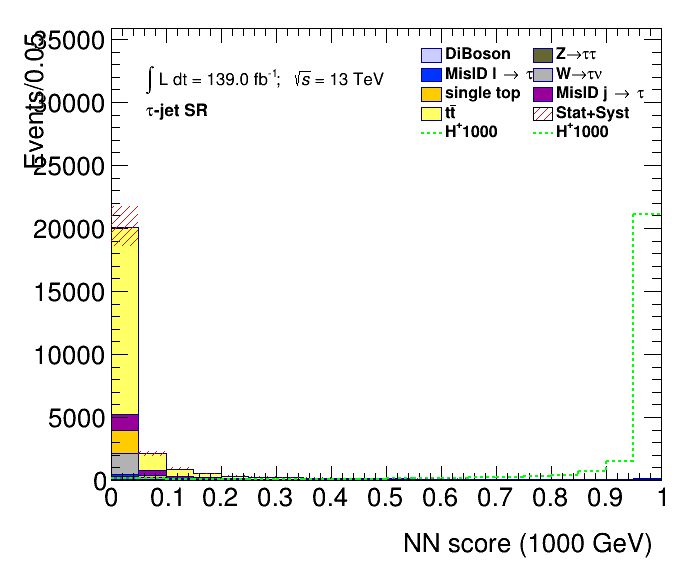
\includegraphics[width=0.45\linewidth]{chapters/chapter6_HPlus/images/taujets/clf_score_GB200_mass_1000to1000_SR_TAUJET.png}}
			\subfloat[\label{fig:taujets_SR_PNNscores_app_5_b}]{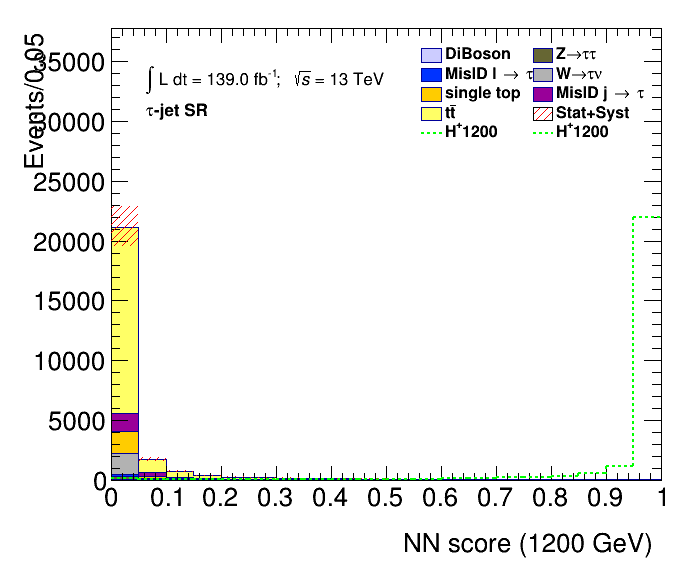
\includegraphics[width=0.45\linewidth]{chapters/chapter6_HPlus/images/taujets/clf_score_GB200_mass_1200to1200_SR_TAUJET.png}} \\
			\subfloat[\label{fig:taujets_SR_PNNscores_app_5_c}]{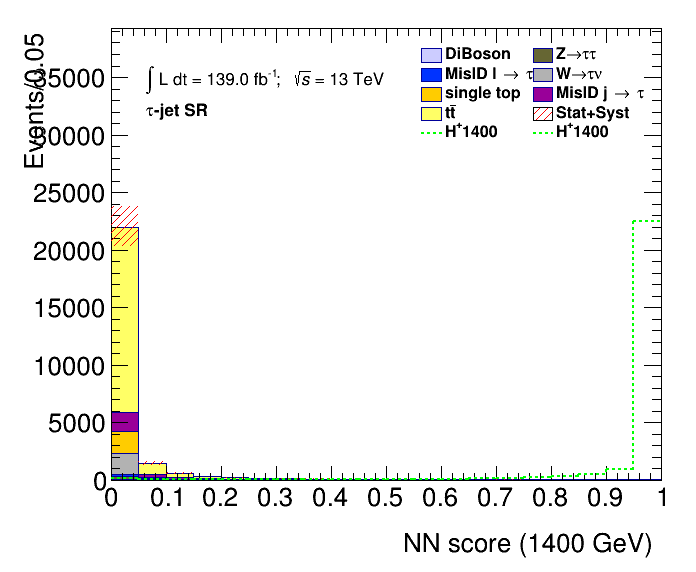
\includegraphics[width=0.45\linewidth]{chapters/chapter6_HPlus/images/taujets/clf_score_GB200_mass_1400to1400_SR_TAUJET.png}}
			\subfloat[\label{fig:taujets_SR_PNNscores_app_5_d}]{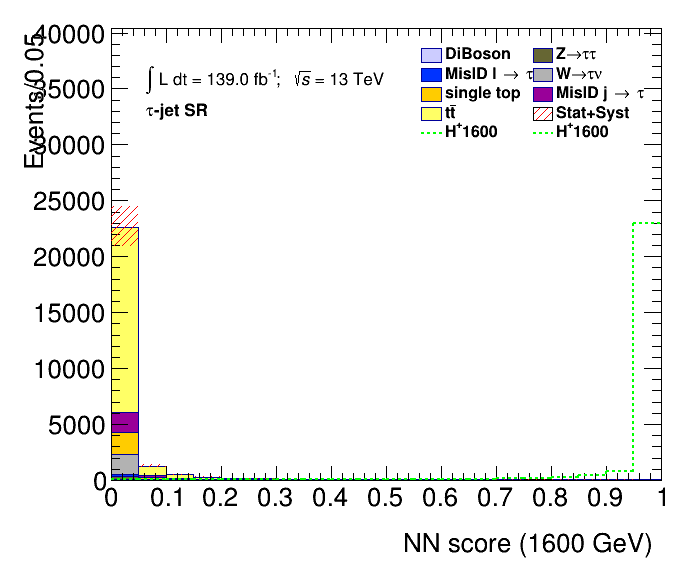
\includegraphics[width=0.45\linewidth]{chapters/chapter6_HPlus/images/taujets/clf_score_GB200_mass_1600to1600_SR_TAUJET.png}} \\
			\subfloat[\label{fig:taujets_SR_PNNscores_app_5_e}]{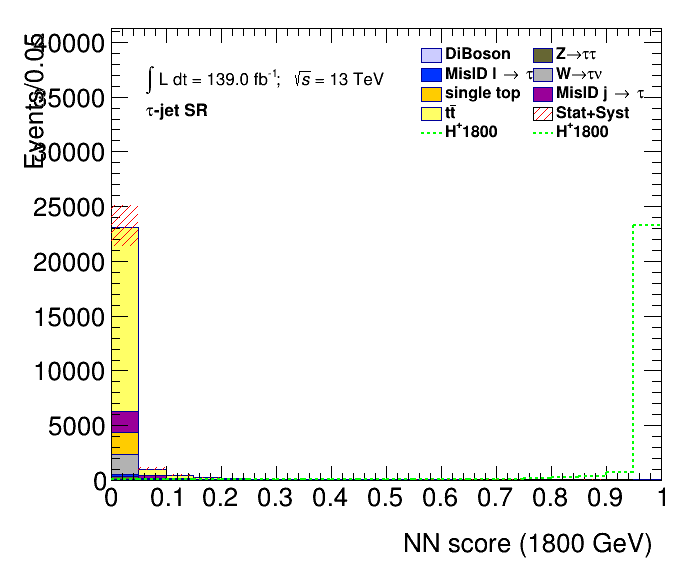
\includegraphics[width=0.45\linewidth]{chapters/chapter6_HPlus/images/taujets/clf_score_GB200_mass_1800to1800_SR_TAUJET.png}}
			\subfloat[\label{fig:taujets_SR_PNNscores_app_5_f}]{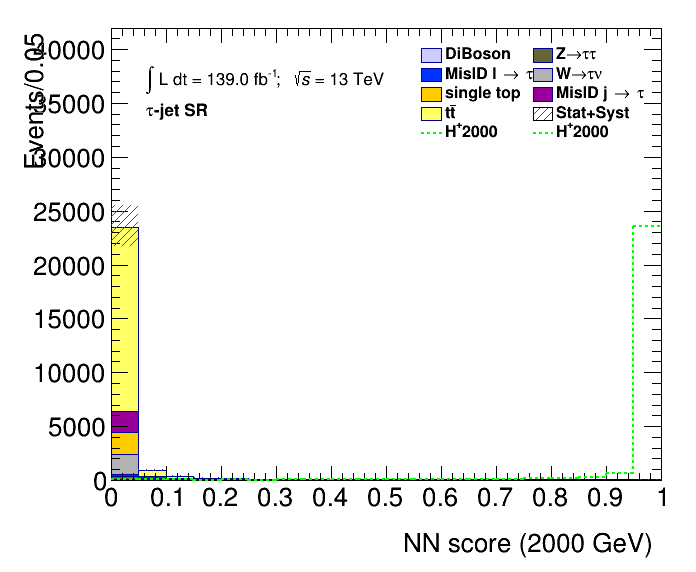
\includegraphics[width=0.45\linewidth]{chapters/chapter6_HPlus/images/taujets/clf_score_GB200_mass_2000to2000_SR_TAUJET.png}}
			  \caption{\label{fig:taujets_SR_PNNscores_app_5} \gls{PNN} score distributions in the
			signal region of the \taujets channel, for the six charged Higgs boson mass parameters.
			 The uncertainty bands include all statistical and systematic uncertainties. 
			The normalization of the signal (shown for illustration) corresponds to the integral of the background.}
		\end{figure}

		\begin{figure}
		  \centering
			\subfloat[\label{fig:taujets_SR_PNNscores_app_6_a}]{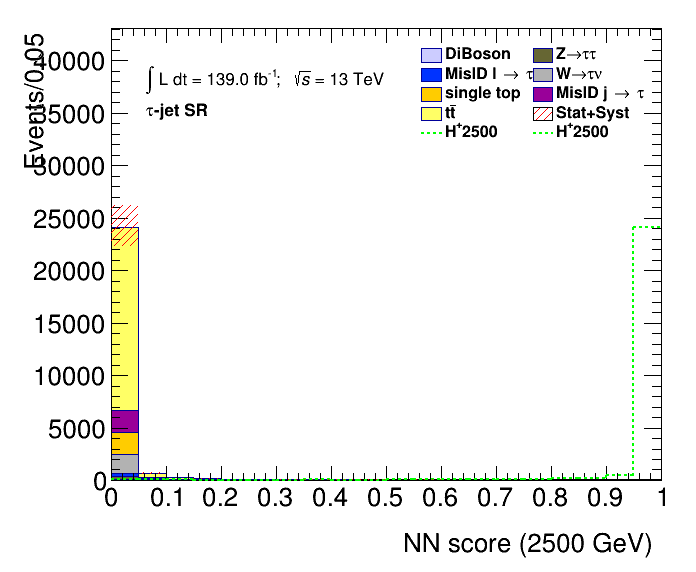
\includegraphics[width=0.45\linewidth]{chapters/chapter6_HPlus/images/taujets/clf_score_GB200_mass_2500to2500_SR_TAUJET.png}}
			\subfloat[\label{fig:taujets_SR_PNNscores_app_6_b}]{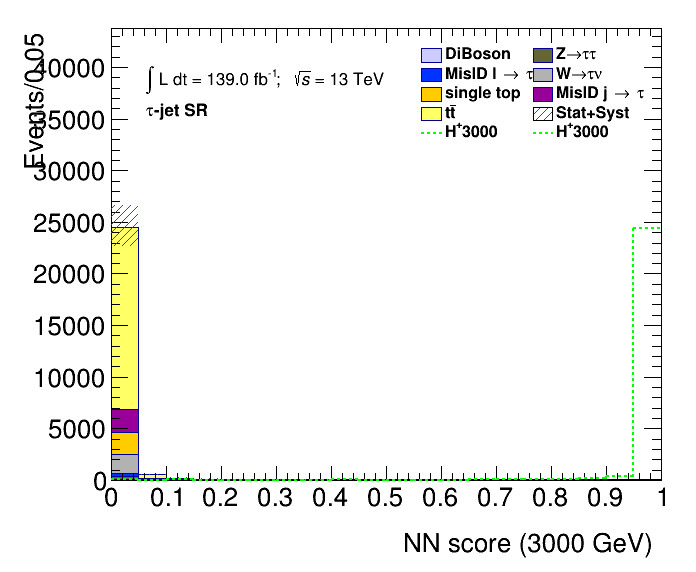
\includegraphics[width=0.45\linewidth]{chapters/chapter6_HPlus/images/taujets/clf_score_GB200_mass_3000to3000_SR_TAUJET.png}} \\
			  \caption{\label{fig:taujets_SR_PNNscores_app_6} \gls{PNN} score distributions in the
			signal region of the \taujets channel, for the six charged Higgs boson mass parameters.
			 The uncertainty bands include all statistical and systematic uncertainties. 
			The normalization of the signal (shown for illustration) corresponds to the integral of the background.}
		\end{figure}

	\clearpage
	\section{\taulep PNN Scores}\label{sec:taulep-pnn-scores}
		\clearpage
		\begin{figure}
		  \centering
			\subfloat[\label{fig:taulep_SR_PNNscores_app_1_a}]{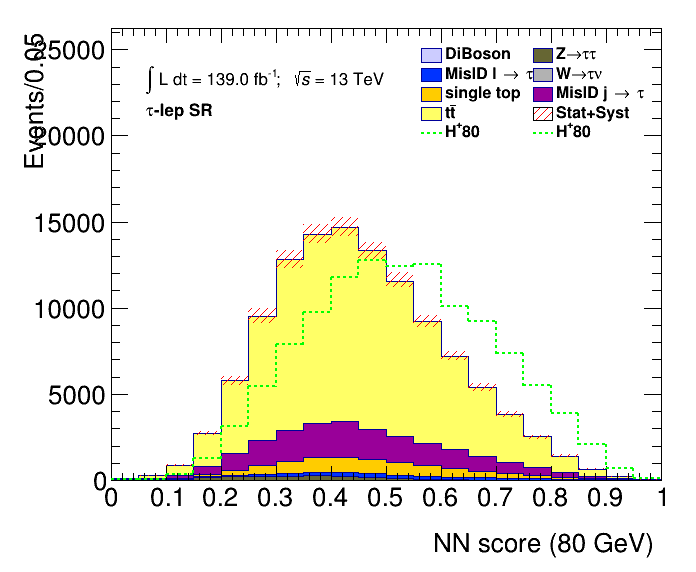
\includegraphics[width=0.45\linewidth]{chapters/chapter6_HPlus/images/taulep/clf_score_GB200_mass_80to80_SR_TAULEP.png}}
			\subfloat[\label{fig:taulep_SR_PNNscores_app_1_b}]{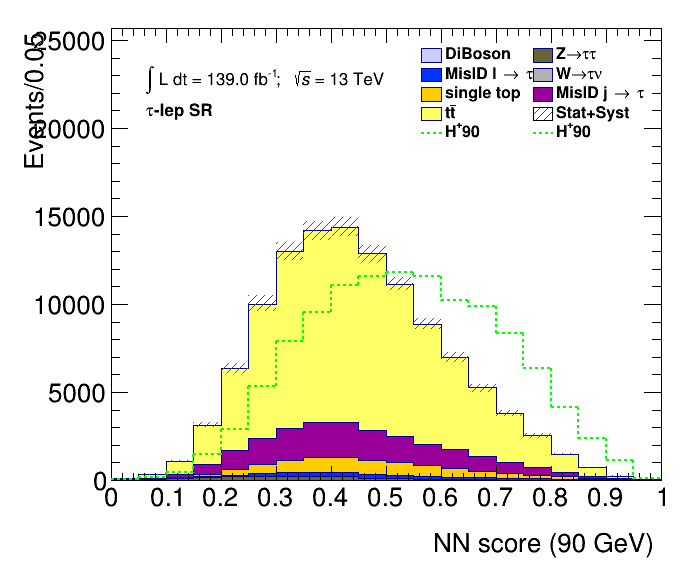
\includegraphics[width=0.45\linewidth]{chapters/chapter6_HPlus/images/taulep/clf_score_GB200_mass_90to90_SR_TAULEP.png}} \\
			\subfloat[\label{fig:taulep_SR_PNNscores_app_1_c}]{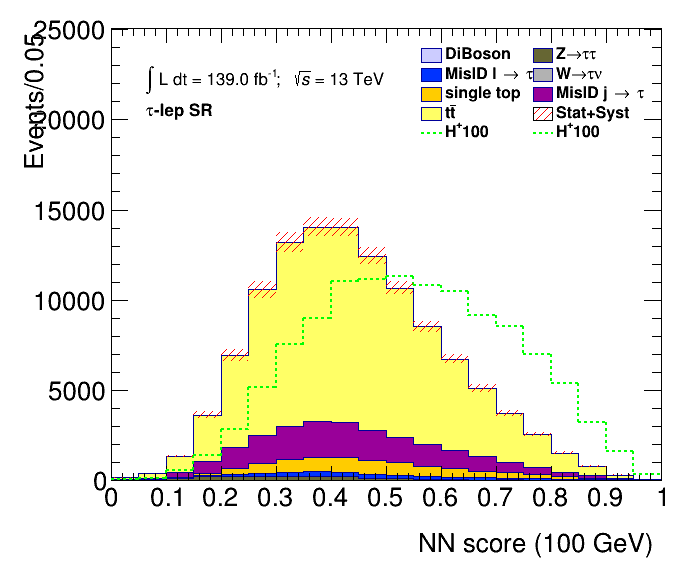
\includegraphics[width=0.45\linewidth]{chapters/chapter6_HPlus/images/taulep/clf_score_GB200_mass_100to100_SR_TAULEP.png}}
			\subfloat[\label{fig:taulep_SR_PNNscores_app_1_d}]{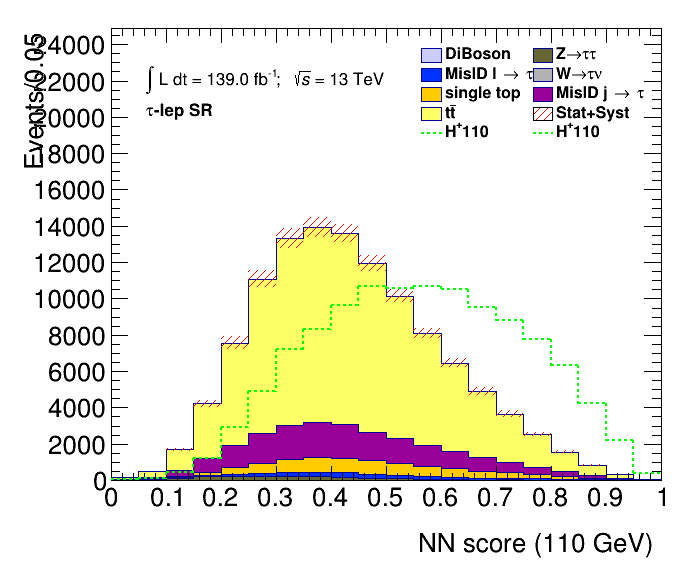
\includegraphics[width=0.45\linewidth]{chapters/chapter6_HPlus/images/taulep/clf_score_GB200_mass_110to110_SR_TAULEP.png}} \\
			\subfloat[\label{fig:taulep_SR_PNNscores_app_1_e}]{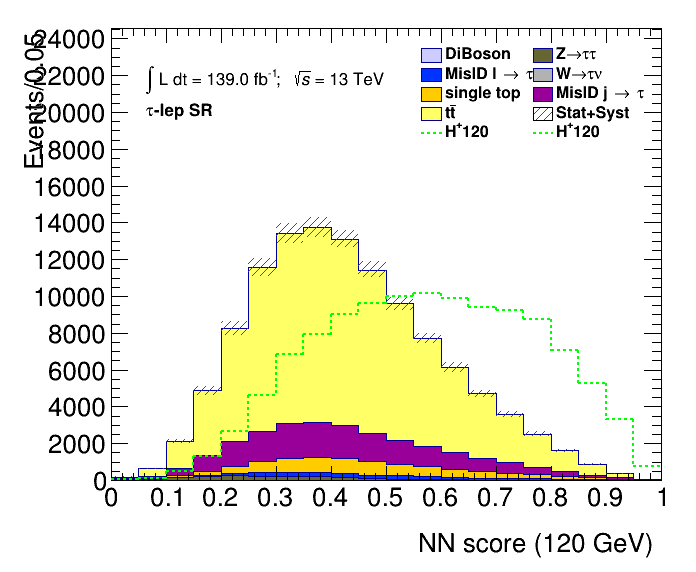
\includegraphics[width=0.45\linewidth]{chapters/chapter6_HPlus/images/taulep/clf_score_GB200_mass_120to120_SR_TAULEP.png}}
			\subfloat[\label{fig:taulep_SR_PNNscores_app_1_f}]{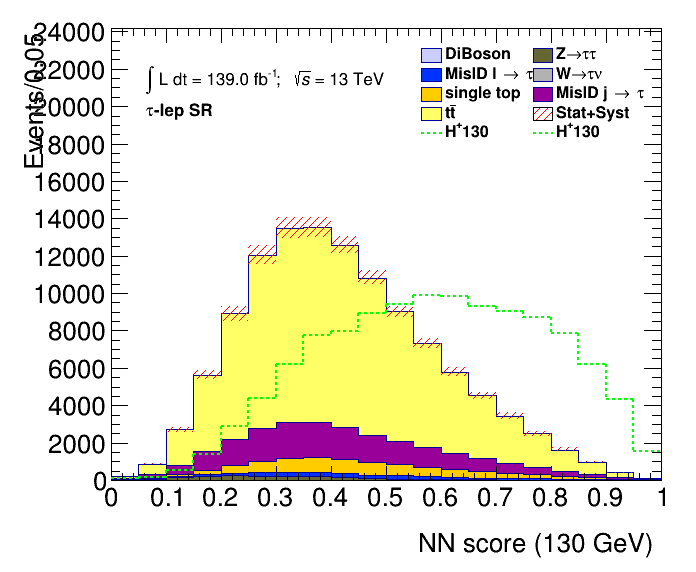
\includegraphics[width=0.45\linewidth]{chapters/chapter6_HPlus/images/taulep/clf_score_GB200_mass_130to130_SR_TAULEP.png}}
			  \caption{\label{fig:taulep_SR_PNNscores_app_1} \gls{PNN} score distributions in the
			signal region of the \taulep channel, for the six charged Higgs boson mass parameters.
			 The uncertainty bands include all statistical and systematic uncertainties. 
			The normalization of the signal (shown for illustration) corresponds to the integral of the background.}
		\end{figure}

		\begin{figure}
		  \centering
			\subfloat[\label{fig:taulep_SR_PNNscores_app_2_a}]{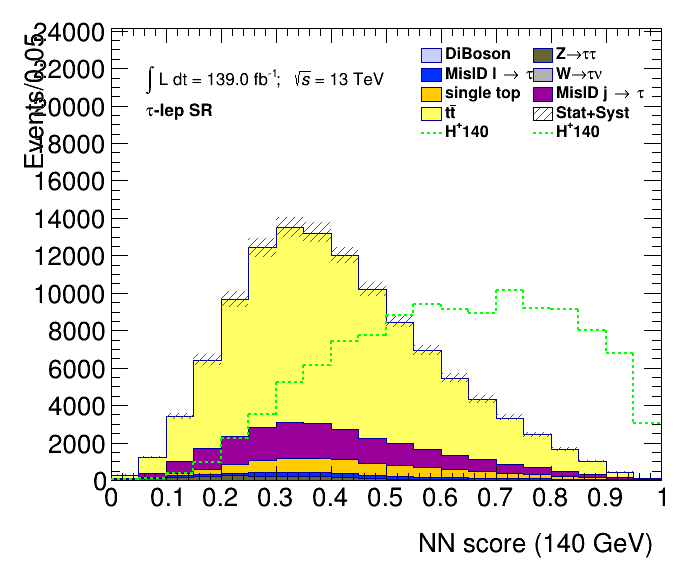
\includegraphics[width=0.45\linewidth]{chapters/chapter6_HPlus/images/taulep/clf_score_GB200_mass_140to140_SR_TAULEP.png}}
			\subfloat[\label{fig:taulep_SR_PNNscores_app_2_b}]{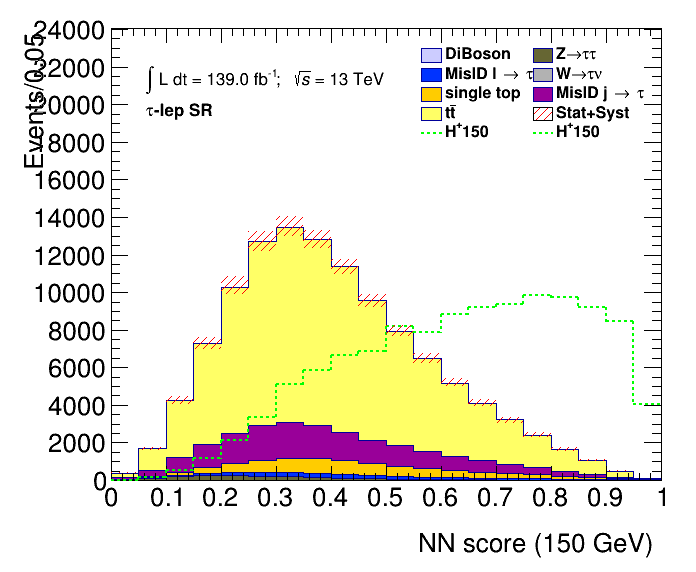
\includegraphics[width=0.45\linewidth]{chapters/chapter6_HPlus/images/taulep/clf_score_GB200_mass_150to150_SR_TAULEP.png}} \\
			\subfloat[\label{fig:taulep_SR_PNNscores_app_2_c}]{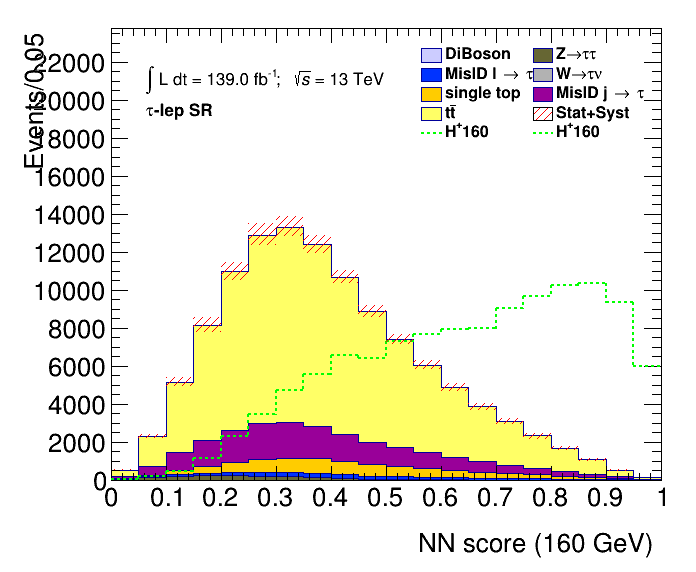
\includegraphics[width=0.45\linewidth]{chapters/chapter6_HPlus/images/taulep/clf_score_GB200_mass_160to160_SR_TAULEP.png}}
			\subfloat[\label{fig:taulep_SR_PNNscores_app_2_d}]{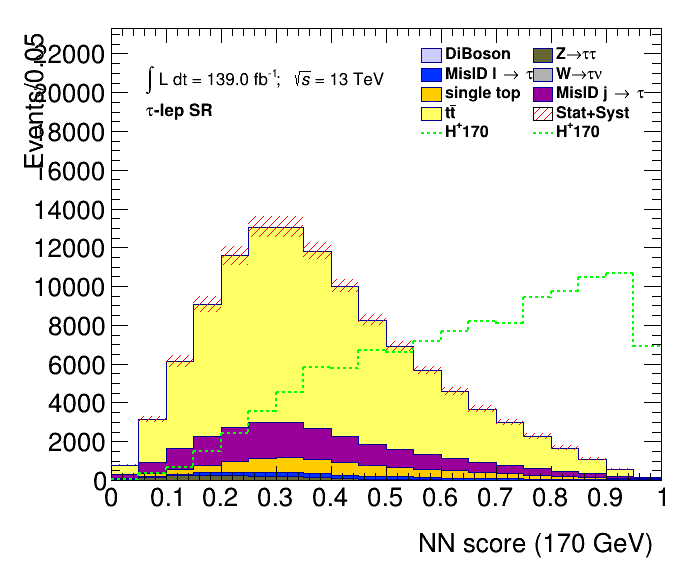
\includegraphics[width=0.45\linewidth]{chapters/chapter6_HPlus/images/taulep/clf_score_GB200_mass_170to170_SR_TAULEP.png}} \\
			\subfloat[\label{fig:taulep_SR_PNNscores_app_2_e}]{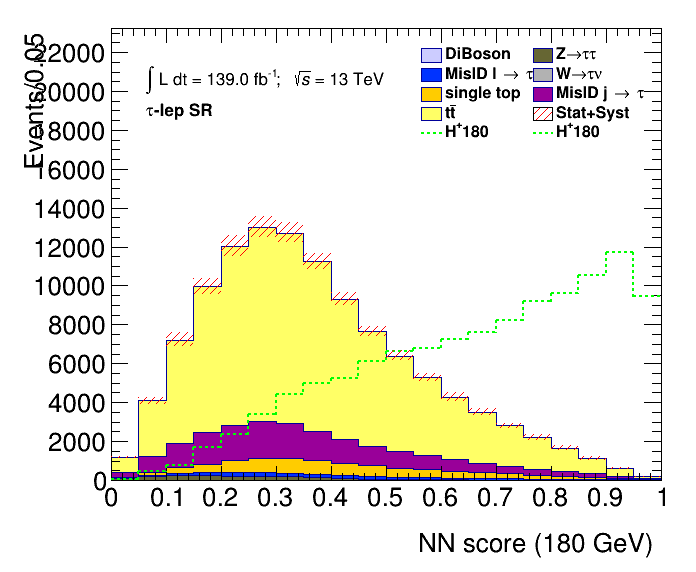
\includegraphics[width=0.45\linewidth]{chapters/chapter6_HPlus/images/taulep/clf_score_GB200_mass_180to180_SR_TAULEP.png}}
			\subfloat[\label{fig:taulep_SR_PNNscores_app_2_f}]{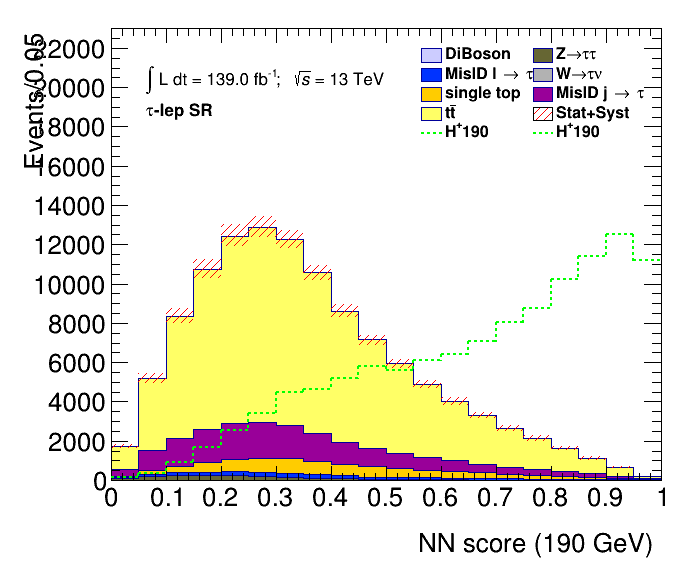
\includegraphics[width=0.45\linewidth]{chapters/chapter6_HPlus/images/taulep/clf_score_GB200_mass_190to190_SR_TAULEP.png}}
			  \caption{\label{fig:taulep_SR_PNNscores_app_2} \gls{PNN} score distributions in the
			signal region of the \taulep channel, for the six charged Higgs boson mass parameters.
			 The uncertainty bands include all statistical and systematic uncertainties. 
			The normalization of the signal (shown for illustration) corresponds to the integral of the background.}
		\end{figure}

		\begin{figure}
		  \centering
			\subfloat[\label{fig:taulep_SR_PNNscores_app_3_a}]{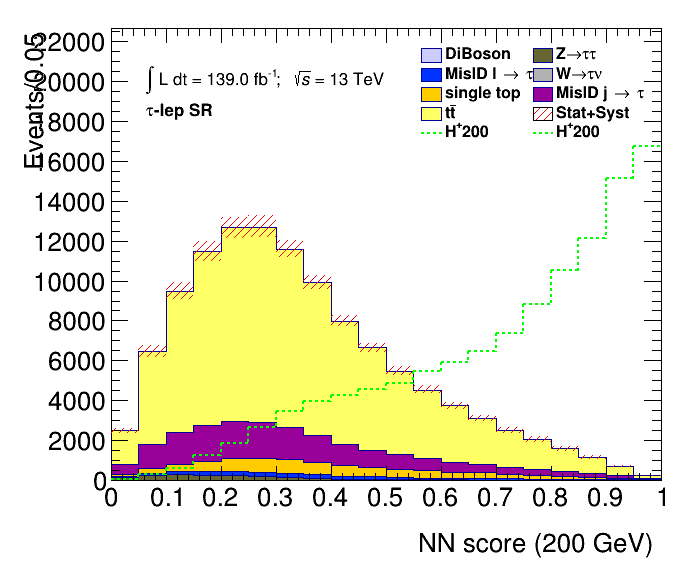
\includegraphics[width=0.45\linewidth]{chapters/chapter6_HPlus/images/taulep/clf_score_GB200_mass_200to200_SR_TAULEP.png}}
			\subfloat[\label{fig:taulep_SR_PNNscores_app_3_b}]{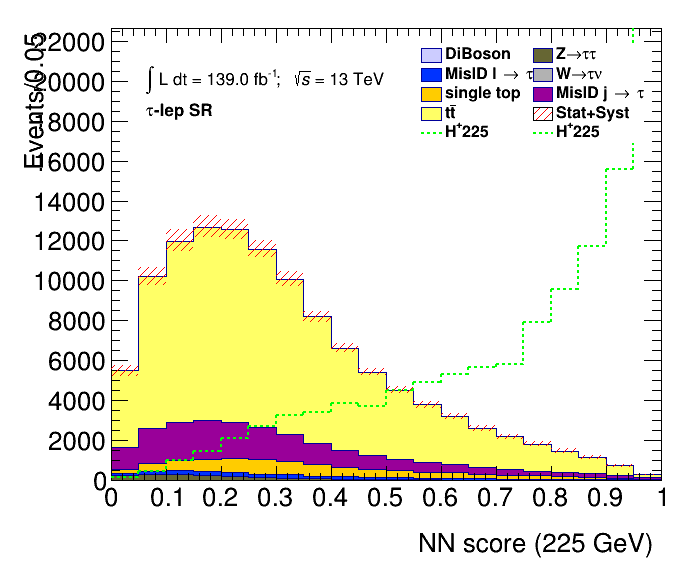
\includegraphics[width=0.45\linewidth]{chapters/chapter6_HPlus/images/taulep/clf_score_GB200_mass_225to225_SR_TAULEP.png}} \\
			\subfloat[\label{fig:taulep_SR_PNNscores_app_3_c}]{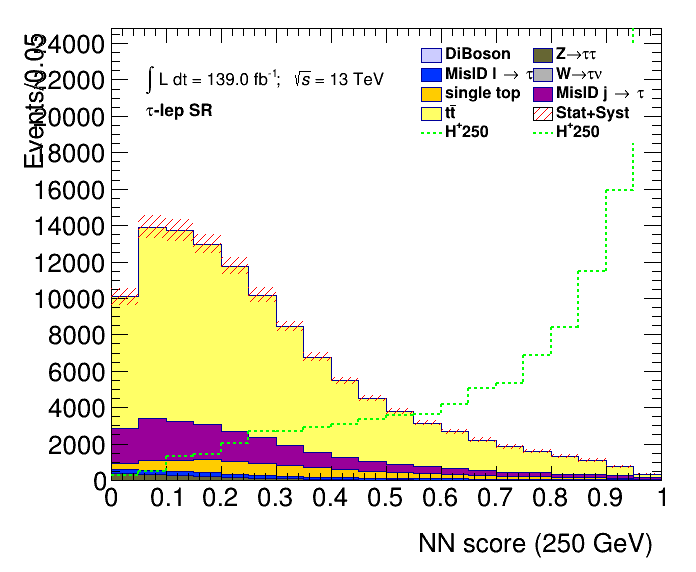
\includegraphics[width=0.45\linewidth]{chapters/chapter6_HPlus/images/taulep/clf_score_GB200_mass_250to250_SR_TAULEP.png}}
			\subfloat[\label{fig:taulep_SR_PNNscores_app_3_d}]{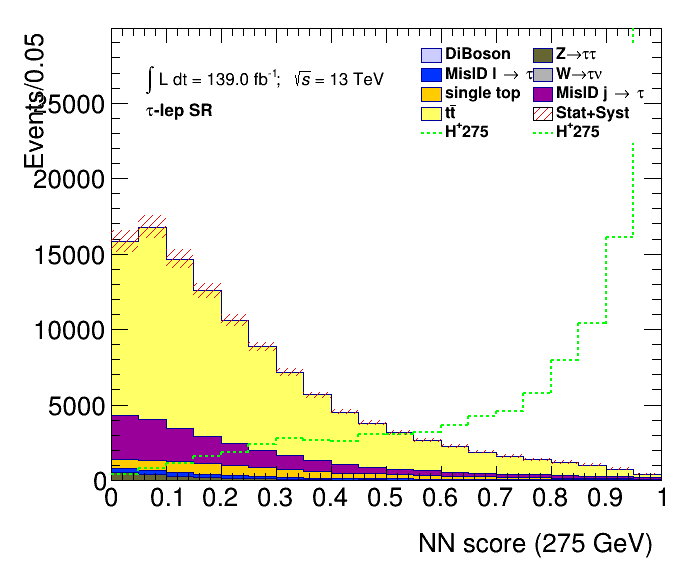
\includegraphics[width=0.45\linewidth]{chapters/chapter6_HPlus/images/taulep/clf_score_GB200_mass_275to275_SR_TAULEP.png}} \\
			\subfloat[\label{fig:taulep_SR_PNNscores_app_3_e}]{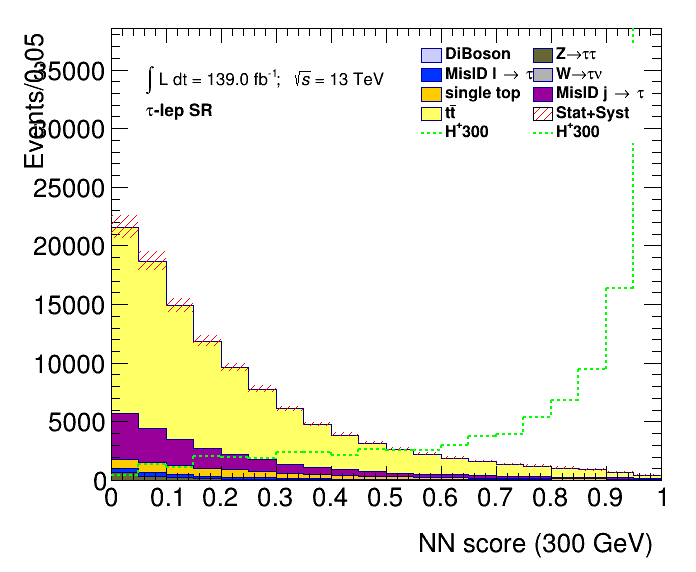
\includegraphics[width=0.45\linewidth]{chapters/chapter6_HPlus/images/taulep/clf_score_GB200_mass_300to300_SR_TAULEP.png}}
			\subfloat[\label{fig:taulep_SR_PNNscores_app_3_f}]{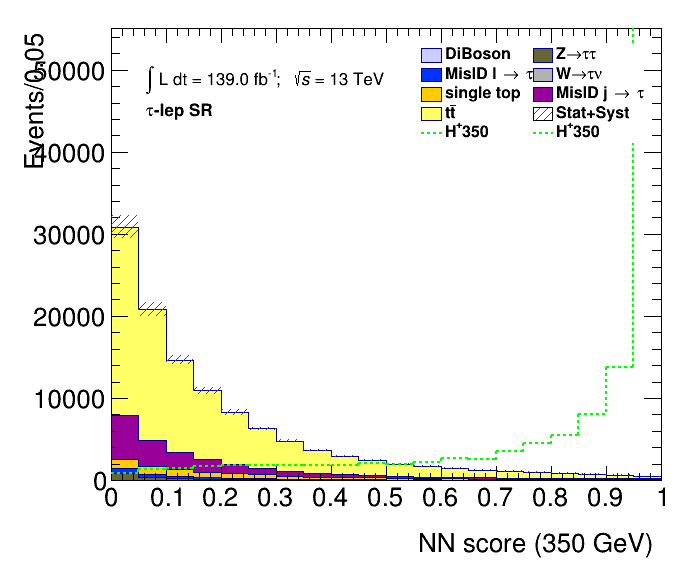
\includegraphics[width=0.45\linewidth]{chapters/chapter6_HPlus/images/taulep/clf_score_GB200_mass_350to350_SR_TAULEP.png}}
			  \caption{\label{fig:taulep_SR_PNNscores_app_3} \gls{PNN} score distributions in the
			signal region of the \taulep channel, for the six charged Higgs boson mass parameters.
			 The uncertainty bands include all statistical and systematic uncertainties. 
			The normalization of the signal (shown for illustration) corresponds to the integral of the background.}
		\end{figure}

		\begin{figure}
		  \centering
			\subfloat[\label{fig:taulep_SR_PNNscores_app_4_a}]{\includegraphics[width=0.45\linewidth]{chapters/chapter6_HPlus/images/taulep/clf_score_GB200_mass_400to400_SR_TAULEP.png}}
			\subfloat[\label{fig:taulep_SR_PNNscores_app_4_b}]{\includegraphics[width=0.45\linewidth]{chapters/chapter6_HPlus/images/taulep/clf_score_GB200_mass_500to500_SR_TAULEP.png}} \\
			\subfloat[\label{fig:taulep_SR_PNNscores_app_4_c}]{\includegraphics[width=0.45\linewidth]{chapters/chapter6_HPlus/images/taulep/clf_score_GB200_mass_600to600_SR_TAULEP.png}}
			\subfloat[\label{fig:taulep_SR_PNNscores_app_4_d}]{\includegraphics[width=0.45\linewidth]{chapters/chapter6_HPlus/images/taulep/clf_score_GB200_mass_700to700_SR_TAULEP.png}} \\
			\subfloat[\label{fig:taulep_SR_PNNscores_app_4_e}]{\includegraphics[width=0.45\linewidth]{chapters/chapter6_HPlus/images/taulep/clf_score_GB200_mass_800to800_SR_TAULEP.png}}
			\subfloat[\label{fig:taulep_SR_PNNscores_app_4_f}]{\includegraphics[width=0.45\linewidth]{chapters/chapter6_HPlus/images/taulep/clf_score_GB200_mass_900to900_SR_TAULEP.png}}
			  \caption{\label{fig:taulep_SR_PNNscores_app_4} \gls{PNN} score distributions in the
			signal region of the \taulep channel, for the six charged Higgs boson mass parameters.
			 The uncertainty bands include all statistical and systematic uncertainties. 
			The normalization of the signal (shown for illustration) corresponds to the integral of the background.}
		\end{figure}

		\begin{figure}
		  \centering
			\subfloat[\label{fig:taulep_SR_PNNscores_app_5_a}]{\includegraphics[width=0.45\linewidth]{chapters/chapter6_HPlus/images/taulep/clf_score_GB200_mass_1000to1000_SR_TAULEP.png}}
			\subfloat[\label{fig:taulep_SR_PNNscores_app_5_b}]{\includegraphics[width=0.45\linewidth]{chapters/chapter6_HPlus/images/taulep/clf_score_GB200_mass_1200to1200_SR_TAULEP.png}} \\
			\subfloat[\label{fig:taulep_SR_PNNscores_app_5_c}]{\includegraphics[width=0.45\linewidth]{chapters/chapter6_HPlus/images/taulep/clf_score_GB200_mass_1400to1400_SR_TAULEP.png}}
			\subfloat[\label{fig:taulep_SR_PNNscores_app_5_d}]{\includegraphics[width=0.45\linewidth]{chapters/chapter6_HPlus/images/taulep/clf_score_GB200_mass_1600to1600_SR_TAULEP.png}} \\
			\subfloat[\label{fig:taulep_SR_PNNscores_app_5_e}]{\includegraphics[width=0.45\linewidth]{chapters/chapter6_HPlus/images/taulep/clf_score_GB200_mass_1800to1800_SR_TAULEP.png}}
			\subfloat[\label{fig:taulep_SR_PNNscores_app_5_f}]{\includegraphics[width=0.45\linewidth]{chapters/chapter6_HPlus/images/taulep/clf_score_GB200_mass_2000to2000_SR_TAULEP.png}}
			  \caption{\label{fig:taulep_SR_PNNscores_app_5} \gls{PNN} score distributions in the
			signal region of the \taulep channel, for the six charged Higgs boson mass parameters.
			 The uncertainty bands include all statistical and systematic uncertainties. 
			The normalization of the signal (shown for illustration) corresponds to the integral of the background.}
		\end{figure}

		\begin{figure}
		  \centering
			\subfloat[\label{fig:taulep_SR_PNNscores_app_6_a}]{\includegraphics[width=0.45\linewidth]{chapters/chapter6_HPlus/images/taulep/clf_score_GB200_mass_2500to2500_SR_TAULEP.png}}
			\subfloat[\label{fig:taulep_SR_PNNscores_app_6_b}]{\includegraphics[width=0.45\linewidth]{chapters/chapter6_HPlus/images/taulep/clf_score_GB200_mass_3000to3000_SR_TAULEP.png}} \\
			  \caption{\label{fig:taulep_SR_PNNscores_app_6} \gls{PNN} score distributions in the
			signal region of the \taulep channel, for the six charged Higgs boson mass parameters.
			 The uncertainty bands include all statistical and systematic uncertainties. 
			The normalization of the signal (shown for illustration) corresponds to the integral of the background.}
		\end{figure}

	\clearpage
	\section{\tauel PNN Scores}\label{sec:tauel-pnn-scores}
		\clearpage
		\begin{figure}
		  \centering
			\subfloat[\label{fig:tauel_SR_PNNscores_app_1_a}]{\includegraphics[width=0.45\linewidth]{chapters/chapter6_HPlus/images/taulep/clf_score_GB200_mass_80to80_SR_TAUEL.png}}
			\subfloat[\label{fig:tauel_SR_PNNscores_app_1_b}]{\includegraphics[width=0.45\linewidth]{chapters/chapter6_HPlus/images/taulep/clf_score_GB200_mass_90to90_SR_TAUEL.png}} \\
			\subfloat[\label{fig:tauel_SR_PNNscores_app_1_c}]{\includegraphics[width=0.45\linewidth]{chapters/chapter6_HPlus/images/taulep/clf_score_GB200_mass_100to100_SR_TAUEL.png}}
			\subfloat[\label{fig:tauel_SR_PNNscores_app_1_d}]{\includegraphics[width=0.45\linewidth]{chapters/chapter6_HPlus/images/taulep/clf_score_GB200_mass_110to110_SR_TAUEL.png}} \\
			\subfloat[\label{fig:tauel_SR_PNNscores_app_1_e}]{\includegraphics[width=0.45\linewidth]{chapters/chapter6_HPlus/images/taulep/clf_score_GB200_mass_120to120_SR_TAUEL.png}}
			\subfloat[\label{fig:tauel_SR_PNNscores_app_1_f}]{\includegraphics[width=0.45\linewidth]{chapters/chapter6_HPlus/images/taulep/clf_score_GB200_mass_130to130_SR_TAUEL.png}}
			  \caption{\label{fig:tauel_SR_PNNscores_app_1} \gls{PNN} score distributions in the
			signal region of the \tauel channel, for the six charged Higgs boson mass parameters.
			 The uncertainty bands include all statistical and systematic uncertainties. 
			The normalization of the signal (shown for illustration) corresponds to the integral of the background.}
		\end{figure}

		\begin{figure}
		  \centering
			\subfloat[\label{fig:tauel_SR_PNNscores_app_2_a}]{\includegraphics[width=0.45\linewidth]{chapters/chapter6_HPlus/images/taulep/clf_score_GB200_mass_140to140_SR_TAUEL.png}}
			\subfloat[\label{fig:tauel_SR_PNNscores_app_2_b}]{\includegraphics[width=0.45\linewidth]{chapters/chapter6_HPlus/images/taulep/clf_score_GB200_mass_150to150_SR_TAUEL.png}} \\
			\subfloat[\label{fig:tauel_SR_PNNscores_app_2_c}]{\includegraphics[width=0.45\linewidth]{chapters/chapter6_HPlus/images/taulep/clf_score_GB200_mass_160to160_SR_TAUEL.png}}
			\subfloat[\label{fig:tauel_SR_PNNscores_app_2_d}]{\includegraphics[width=0.45\linewidth]{chapters/chapter6_HPlus/images/taulep/clf_score_GB200_mass_170to170_SR_TAUEL.png}} \\
			\subfloat[\label{fig:tauel_SR_PNNscores_app_2_e}]{\includegraphics[width=0.45\linewidth]{chapters/chapter6_HPlus/images/taulep/clf_score_GB200_mass_180to180_SR_TAUEL.png}}
			\subfloat[\label{fig:tauel_SR_PNNscores_app_2_f}]{\includegraphics[width=0.45\linewidth]{chapters/chapter6_HPlus/images/taulep/clf_score_GB200_mass_190to190_SR_TAUEL.png}}
			  \caption{\label{fig:tauel_SR_PNNscores_app_2} \gls{PNN} score distributions in the
			signal region of the \tauel channel, for the six charged Higgs boson mass parameters.
			 The uncertainty bands include all statistical and systematic uncertainties. 
			The normalization of the signal (shown for illustration) corresponds to the integral of the background.}
		\end{figure}

		\begin{figure}
		  \centering
			\subfloat[\label{fig:tauel_SR_PNNscores_app_3_a}]{\includegraphics[width=0.45\linewidth]{chapters/chapter6_HPlus/images/taulep/clf_score_GB200_mass_200to200_SR_TAUEL.png}}
			\subfloat[\label{fig:tauel_SR_PNNscores_app_3_b}]{\includegraphics[width=0.45\linewidth]{chapters/chapter6_HPlus/images/taulep/clf_score_GB200_mass_225to225_SR_TAUEL.png}} \\
			\subfloat[\label{fig:tauel_SR_PNNscores_app_3_c}]{\includegraphics[width=0.45\linewidth]{chapters/chapter6_HPlus/images/taulep/clf_score_GB200_mass_250to250_SR_TAUEL.png}}
			\subfloat[\label{fig:tauel_SR_PNNscores_app_3_d}]{\includegraphics[width=0.45\linewidth]{chapters/chapter6_HPlus/images/taulep/clf_score_GB200_mass_275to275_SR_TAUEL.png}} \\
			\subfloat[\label{fig:tauel_SR_PNNscores_app_3_e}]{\includegraphics[width=0.45\linewidth]{chapters/chapter6_HPlus/images/taulep/clf_score_GB200_mass_300to300_SR_TAUEL.png}}
			\subfloat[\label{fig:tauel_SR_PNNscores_app_3_f}]{\includegraphics[width=0.45\linewidth]{chapters/chapter6_HPlus/images/taulep/clf_score_GB200_mass_350to350_SR_TAUEL.png}}
			  \caption{\label{fig:tauel_SR_PNNscores_app_3} \gls{PNN} score distributions in the
			signal region of the \tauel channel, for the six charged Higgs boson mass parameters.
			 The uncertainty bands include all statistical and systematic uncertainties. 
			The normalization of the signal (shown for illustration) corresponds to the integral of the background.}
		\end{figure}

		\begin{figure}
		  \centering
			\subfloat[\label{fig:tauel_SR_PNNscores_app_4_a}]{\includegraphics[width=0.45\linewidth]{chapters/chapter6_HPlus/images/taulep/clf_score_GB200_mass_400to400_SR_TAUEL.png}}
			\subfloat[\label{fig:tauel_SR_PNNscores_app_4_b}]{\includegraphics[width=0.45\linewidth]{chapters/chapter6_HPlus/images/taulep/clf_score_GB200_mass_500to500_SR_TAUEL.png}} \\
			\subfloat[\label{fig:tauel_SR_PNNscores_app_4_c}]{\includegraphics[width=0.45\linewidth]{chapters/chapter6_HPlus/images/taulep/clf_score_GB200_mass_600to600_SR_TAUEL.png}}
			\subfloat[\label{fig:tauel_SR_PNNscores_app_4_d}]{\includegraphics[width=0.45\linewidth]{chapters/chapter6_HPlus/images/taulep/clf_score_GB200_mass_700to700_SR_TAUEL.png}} \\
			\subfloat[\label{fig:tauel_SR_PNNscores_app_4_e}]{\includegraphics[width=0.45\linewidth]{chapters/chapter6_HPlus/images/taulep/clf_score_GB200_mass_800to800_SR_TAUEL.png}}
			\subfloat[\label{fig:tauel_SR_PNNscores_app_4_f}]{\includegraphics[width=0.45\linewidth]{chapters/chapter6_HPlus/images/taulep/clf_score_GB200_mass_900to900_SR_TAUEL.png}}
			  \caption{\label{fig:tauel_SR_PNNscores_app_4} \gls{PNN} score distributions in the
			signal region of the \tauel channel, for the six charged Higgs boson mass parameters.
			 The uncertainty bands include all statistical and systematic uncertainties. 
			The normalization of the signal (shown for illustration) corresponds to the integral of the background.}
		\end{figure}

		\begin{figure}
		  \centering
			\subfloat[\label{fig:tauel_SR_PNNscores_app_5_a}]{\includegraphics[width=0.45\linewidth]{chapters/chapter6_HPlus/images/taulep/clf_score_GB200_mass_1000to1000_SR_TAUEL.png}}
			\subfloat[\label{fig:tauel_SR_PNNscores_app_5_b}]{\includegraphics[width=0.45\linewidth]{chapters/chapter6_HPlus/images/taulep/clf_score_GB200_mass_1200to1200_SR_TAUEL.png}} \\
			\subfloat[\label{fig:tauel_SR_PNNscores_app_5_c}]{\includegraphics[width=0.45\linewidth]{chapters/chapter6_HPlus/images/taulep/clf_score_GB200_mass_1400to1400_SR_TAUEL.png}}
			\subfloat[\label{fig:tauel_SR_PNNscores_app_5_d}]{\includegraphics[width=0.45\linewidth]{chapters/chapter6_HPlus/images/taulep/clf_score_GB200_mass_1600to1600_SR_TAUEL.png}} \\
			\subfloat[\label{fig:tauel_SR_PNNscores_app_5_e}]{\includegraphics[width=0.45\linewidth]{chapters/chapter6_HPlus/images/taulep/clf_score_GB200_mass_1800to1800_SR_TAUEL.png}}
			\subfloat[\label{fig:tauel_SR_PNNscores_app_5_f}]{\includegraphics[width=0.45\linewidth]{chapters/chapter6_HPlus/images/taulep/clf_score_GB200_mass_2000to2000_SR_TAUEL.png}}
			  \caption{\label{fig:tauel_SR_PNNscores_app_5} \gls{PNN} score distributions in the
			signal region of the \tauel channel, for the six charged Higgs boson mass parameters.
			 The uncertainty bands include all statistical and systematic uncertainties. 
			The normalization of the signal (shown for illustration) corresponds to the integral of the background.}
		\end{figure}

		\begin{figure}
		  \centering
			\subfloat[\label{fig:tauel_SR_PNNscores_app_6_a}]{\includegraphics[width=0.45\linewidth]{chapters/chapter6_HPlus/images/taulep/clf_score_GB200_mass_2500to2500_SR_TAUEL.png}}
			\subfloat[\label{fig:tauel_SR_PNNscores_app_6_b}]{\includegraphics[width=0.45\linewidth]{chapters/chapter6_HPlus/images/taulep/clf_score_GB200_mass_3000to3000_SR_TAUEL.png}} \\
			  \caption{\label{fig:tauel_SR_PNNscores_app_6} \gls{PNN} score distributions in the
			signal region of the \tauel channel, for the six charged Higgs boson mass parameters.
			 The uncertainty bands include all statistical and systematic uncertainties. 
			The normalization of the signal (shown for illustration) corresponds to the integral of the background.}
		\end{figure}

	\clearpage
	\section{\taumu PNN Scores}\label{sec:taumu-pnn-scores}
		\clearpage
		\begin{figure}
		  \centering
			\subfloat[\label{fig:taumu_SR_PNNscores_app_1_a}]{\includegraphics[width=0.45\linewidth]{chapters/chapter6_HPlus/images/taulep/clf_score_GB200_mass_80to80_SR_TAUMU.png}}
			\subfloat[\label{fig:taumu_SR_PNNscores_app_1_b}]{\includegraphics[width=0.45\linewidth]{chapters/chapter6_HPlus/images/taulep/clf_score_GB200_mass_90to90_SR_TAUMU.png}} \\
			\subfloat[\label{fig:taumu_SR_PNNscores_app_1_c}]{\includegraphics[width=0.45\linewidth]{chapters/chapter6_HPlus/images/taulep/clf_score_GB200_mass_100to100_SR_TAUMU.png}}
			\subfloat[\label{fig:taumu_SR_PNNscores_app_1_d}]{\includegraphics[width=0.45\linewidth]{chapters/chapter6_HPlus/images/taulep/clf_score_GB200_mass_110to110_SR_TAUMU.png}} \\
			\subfloat[\label{fig:taumu_SR_PNNscores_app_1_e}]{\includegraphics[width=0.45\linewidth]{chapters/chapter6_HPlus/images/taulep/clf_score_GB200_mass_120to120_SR_TAUMU.png}}
			\subfloat[\label{fig:taumu_SR_PNNscores_app_1_f}]{\includegraphics[width=0.45\linewidth]{chapters/chapter6_HPlus/images/taulep/clf_score_GB200_mass_130to130_SR_TAUMU.png}}
			  \caption{\label{fig:taumu_SR_PNNscores_app_1} \gls{PNN} score distributions in the
			signal region of the \taumu channel, for the six charged Higgs boson mass parameters.
			 The uncertainty bands include all statistical and systematic uncertainties. 
			The normalization of the signal (shown for illustration) corresponds to the integral of the background.}
		\end{figure}

		\begin{figure}
		  \centering
			\subfloat[\label{fig:taumu_SR_PNNscores_app_2_a}]{\includegraphics[width=0.45\linewidth]{chapters/chapter6_HPlus/images/taulep/clf_score_GB200_mass_140to140_SR_TAUMU.png}}
			\subfloat[\label{fig:taumu_SR_PNNscores_app_2_b}]{\includegraphics[width=0.45\linewidth]{chapters/chapter6_HPlus/images/taulep/clf_score_GB200_mass_150to150_SR_TAUMU.png}} \\
			\subfloat[\label{fig:taumu_SR_PNNscores_app_2_c}]{\includegraphics[width=0.45\linewidth]{chapters/chapter6_HPlus/images/taulep/clf_score_GB200_mass_160to160_SR_TAUMU.png}}
			\subfloat[\label{fig:taumu_SR_PNNscores_app_2_d}]{\includegraphics[width=0.45\linewidth]{chapters/chapter6_HPlus/images/taulep/clf_score_GB200_mass_170to170_SR_TAUMU.png}} \\
			\subfloat[\label{fig:taumu_SR_PNNscores_app_2_e}]{\includegraphics[width=0.45\linewidth]{chapters/chapter6_HPlus/images/taulep/clf_score_GB200_mass_180to180_SR_TAUMU.png}}
			\subfloat[\label{fig:taumu_SR_PNNscores_app_2_f}]{\includegraphics[width=0.45\linewidth]{chapters/chapter6_HPlus/images/taulep/clf_score_GB200_mass_190to190_SR_TAUMU.png}}
			  \caption{\label{fig:taumu_SR_PNNscores_app_2} \gls{PNN} score distributions in the
			signal region of the \taumu channel, for the six charged Higgs boson mass parameters.
			 The uncertainty bands include all statistical and systematic uncertainties. 
			The normalization of the signal (shown for illustration) corresponds to the integral of the background.}
		\end{figure}

		\begin{figure}
		  \centering
			\subfloat[\label{fig:taumu_SR_PNNscores_app_3_a}]{\includegraphics[width=0.45\linewidth]{chapters/chapter6_HPlus/images/taulep/clf_score_GB200_mass_200to200_SR_TAUMU.png}}
			\subfloat[\label{fig:taumu_SR_PNNscores_app_3_b}]{\includegraphics[width=0.45\linewidth]{chapters/chapter6_HPlus/images/taulep/clf_score_GB200_mass_225to225_SR_TAUMU.png}} \\
			\subfloat[\label{fig:taumu_SR_PNNscores_app_3_c}]{\includegraphics[width=0.45\linewidth]{chapters/chapter6_HPlus/images/taulep/clf_score_GB200_mass_250to250_SR_TAUMU.png}}
			\subfloat[\label{fig:taumu_SR_PNNscores_app_3_d}]{\includegraphics[width=0.45\linewidth]{chapters/chapter6_HPlus/images/taulep/clf_score_GB200_mass_275to275_SR_TAUMU.png}} \\
			\subfloat[\label{fig:taumu_SR_PNNscores_app_3_e}]{\includegraphics[width=0.45\linewidth]{chapters/chapter6_HPlus/images/taulep/clf_score_GB200_mass_300to300_SR_TAUMU.png}}
			\subfloat[\label{fig:taumu_SR_PNNscores_app_3_f}]{\includegraphics[width=0.45\linewidth]{chapters/chapter6_HPlus/images/taulep/clf_score_GB200_mass_350to350_SR_TAUMU.png}}
			  \caption{\label{fig:taumu_SR_PNNscores_app_3} \gls{PNN} score distributions in the
			signal region of the \taumu channel, for the six charged Higgs boson mass parameters.
			 The uncertainty bands include all statistical and systematic uncertainties. 
			The normalization of the signal (shown for illustration) corresponds to the integral of the background.}
		\end{figure}

		\begin{figure}
		  \centering
			\subfloat[\label{fig:taumu_SR_PNNscores_app_4_a}]{\includegraphics[width=0.45\linewidth]{chapters/chapter6_HPlus/images/taulep/clf_score_GB200_mass_400to400_SR_TAUMU.png}}
			\subfloat[\label{fig:taumu_SR_PNNscores_app_4_b}]{\includegraphics[width=0.45\linewidth]{chapters/chapter6_HPlus/images/taulep/clf_score_GB200_mass_500to500_SR_TAUMU.png}} \\
			\subfloat[\label{fig:taumu_SR_PNNscores_app_4_c}]{\includegraphics[width=0.45\linewidth]{chapters/chapter6_HPlus/images/taulep/clf_score_GB200_mass_600to600_SR_TAUMU.png}}
			\subfloat[\label{fig:taumu_SR_PNNscores_app_4_d}]{\includegraphics[width=0.45\linewidth]{chapters/chapter6_HPlus/images/taulep/clf_score_GB200_mass_700to700_SR_TAUMU.png}} \\
			\subfloat[\label{fig:taumu_SR_PNNscores_app_4_e}]{\includegraphics[width=0.45\linewidth]{chapters/chapter6_HPlus/images/taulep/clf_score_GB200_mass_800to800_SR_TAUMU.png}}
			\subfloat[\label{fig:taumu_SR_PNNscores_app_4_f}]{\includegraphics[width=0.45\linewidth]{chapters/chapter6_HPlus/images/taulep/clf_score_GB200_mass_900to900_SR_TAUMU.png}}
			  \caption{\label{fig:taumu_SR_PNNscores_app_4} \gls{PNN} score distributions in the
			signal region of the \taumu channel, for the six charged Higgs boson mass parameters.
			 The uncertainty bands include all statistical and systematic uncertainties. 
			The normalization of the signal (shown for illustration) corresponds to the integral of the background.}
		\end{figure}

		\begin{figure}
		  \centering
			\subfloat[\label{fig:taumu_SR_PNNscores_app_5_a}]{\includegraphics[width=0.45\linewidth]{chapters/chapter6_HPlus/images/taulep/clf_score_GB200_mass_1000to1000_SR_TAUMU.png}}
			\subfloat[\label{fig:taumu_SR_PNNscores_app_5_b}]{\includegraphics[width=0.45\linewidth]{chapters/chapter6_HPlus/images/taulep/clf_score_GB200_mass_1200to1200_SR_TAUMU.png}} \\
			\subfloat[\label{fig:taumu_SR_PNNscores_app_5_c}]{\includegraphics[width=0.45\linewidth]{chapters/chapter6_HPlus/images/taulep/clf_score_GB200_mass_1400to1400_SR_TAUMU.png}}
			\subfloat[\label{fig:taumu_SR_PNNscores_app_5_d}]{\includegraphics[width=0.45\linewidth]{chapters/chapter6_HPlus/images/taulep/clf_score_GB200_mass_1600to1600_SR_TAUMU.png}} \\
			\subfloat[\label{fig:taumu_SR_PNNscores_app_5_e}]{\includegraphics[width=0.45\linewidth]{chapters/chapter6_HPlus/images/taulep/clf_score_GB200_mass_1800to1800_SR_TAUMU.png}}
			\subfloat[\label{fig:taumu_SR_PNNscores_app_5_f}]{\includegraphics[width=0.45\linewidth]{chapters/chapter6_HPlus/images/taulep/clf_score_GB200_mass_2000to2000_SR_TAUMU.png}}
			  \caption{\label{fig:taumu_SR_PNNscores_app_5} \gls{PNN} score distributions in the
			signal region of the \taumu channel, for the six charged Higgs boson mass parameters.
			 The uncertainty bands include all statistical and systematic uncertainties. 
			The normalization of the signal (shown for illustration) corresponds to the integral of the background.}
		\end{figure}

		\begin{figure}
		  \centering
			\subfloat[\label{fig:taumu_SR_PNNscores_app_6_a}]{\includegraphics[width=0.45\linewidth]{chapters/chapter6_HPlus/images/taulep/clf_score_GB200_mass_2500to2500_SR_TAUMU.png}}
			\subfloat[\label{fig:taumu_SR_PNNscores_app_6_b}]{\includegraphics[width=0.45\linewidth]{chapters/chapter6_HPlus/images/taulep/clf_score_GB200_mass_3000to3000_SR_TAUMU.png}} \\
			  \caption{\label{fig:taumu_SR_PNNscores_app_6} \gls{PNN} score distributions in the
			signal region of the \taumu channel, for the six charged Higgs boson mass parameters.
			 The uncertainty bands include all statistical and systematic uncertainties. 
			The normalization of the signal (shown for illustration) corresponds to the integral of the background.}
		\end{figure}